\chapter{Quantitative analysis of Lightning network privacy}

\label{Chapter07LNattacks}

We evaluate the possibility of various attacks on Lightning, considering various subsets of nodes potentially compromised.

\todo[inline]{Update with camera-ready version}
\todo[inline]{Split between Chapter 05, 07,08}

Payment channel networks have been introduced to mitigate the scalability issues inherent to permissionless decentralized cryptocurrencies such as Bitcoin.
Launched in 2018, the Lightning Network (LN) has 
been gaining popularity and 
consists today of more than $5000$ nodes and $30000$ payment channels 
that jointly hold $895$~bitcoins ($7.6M$~USD as of February~2020).
This adoption has motivated research from both academia and industry.

Payment channels suffer from security vulnerabilities, such as the wormhole attack~\cite{Malavolta2019}, anonymity issues~\cite{Malavolta2017}, and scalability limitations related to  the upper bound on the number of concurrent payments per channel~\cite{EmelyanenkoK2017}, which have been pointed out by the scientific community but never quantitatively analyzed. 

In this work, we first analyze the proneness of the LN to the wormhole attack and attacks against anonymity. 
We observe that an adversary needs to control only $2\%$ of LN nodes to learn sensitive payment information (e.g., sender, receiver and payment amount) or to carry out the wormhole attack. 
Second, we study the management of concurrent payments in the LN and quantify its negative effect on scalability. 
We observe that for micropayments, the forwarding capability of up to $50\%$ of channels is restricted to 
a value smaller than the overall channel capacity.
This phenomenon not only hinders scalability but also opens the door for DoS attacks: We estimate that 
a network-wide DoS attack costs within $1.5M$~USD, while isolating the biggest community from the rest of the network costs only $225k$~USD.

Our findings should prompt the LN community to consider the security, privacy and scalability issues of the network studied in this work 
when educating users about path selection algorithms, as well as to adopt multi-hop payment protocols that provide stronger security, privacy and 
scalability guarantees. 

\section{Background}
\label{sec:background}

\begin{figure*}[tb]
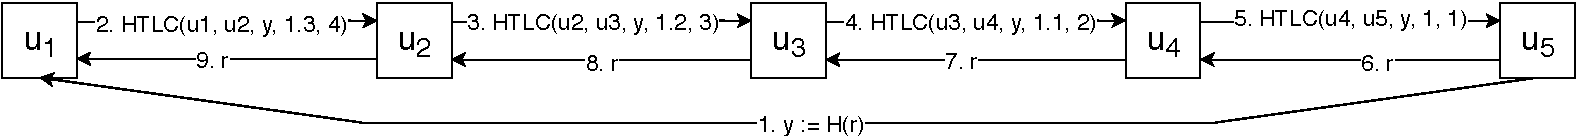
\includegraphics[width=\textwidth]{htlc-figure}
	\caption{An HTLC-based payment in the LN. The node $u_1$ pays $u_5$ using $u_2$, $u_3$ and $u_4$ as intermediaries. 
	Here we assume that each node charges a fee of $0.1$ and time is measured in days.\label{fig:htlc}}
\end{figure*}

The Lightning Network (LN) has emerged as the alternative to the scalability issue of Bitcoin  with the highest adoption in practice~\cite{Cuen2019}.
%LN has experienced rapid growth since its launch in early 2018~, 
As of February~2020, LN facilitates the off-chain exchange of nearly $900$~BTC.
The principles of the LN can be used to improve the scalability of other cryptocurrencies. 
For instance, similar networks operate with Litecoin~\cite{1MLLitecoin} and Ethereum~\cite{RaidenWebsite}. 
In this section, we introduce the basic notions of the LN and refer the reader 
to~\cite{Gudgeon2019} for further reading.
% TowardsBitcoinPaymentNetworks, BitcoinMagazineUnderstandingLightning, 

\subsubsection*{LN nodes} A node in the LN is governed by a pair of signing and verification keys from 
the ECDSA signature scheme, 
and identified by the hashed value of the verification key.  
Additionally, the owner can assign a handcrafted identifier (alias) to their node.
Operations from a node are authorized with a digital signature 
created with the corresponding signing key.
Thus, whoever holds the signing key is the owner of a node.
One user can potentially own several nodes.

%\vspace{-0.2cm}
\subsubsection*{LN channels} A LN channel (i.e.,~an edge) is jointly controlled by the two counterparties and its capacity is determined by the amount of coins 
deposited when created.
While the total capacity of the channel stays constant during its lifetime,
the balance of each counterparty varies according to two operations:
(i) single channel updates, where the two users agree on an updated balance; and 
(ii) multi-hop transactions, where the balance 
of several channels forming a path are simultaneously updated. 

%\vspace{-0.2cm}
\subsubsection*{LN transactions} A multi-hop transaction (or simply a transaction hereby) leverages a 
path of channels between a sender and a receiver (who might not share a channel between them).
A transaction must ensure the atomicity of the transfer: 
either all balances along the path are updated or none of them are.
For that, the LN relies on Hash Time-Lock Contracts (HTLCs), 
 excerpts from the  Bitcoin's scripting language that 
permit a node ($u_1$) to lock $x$~coins in a channel between two nodes ($u_1$ and $u_2$) 
and release them according to the encoded conditions.
The terms for the HTLC($u_1, u_2, y, x, t$) are defined with a hash value $y := H(r)$, 
where $r$ is chosen uniformly at random, 
an amount $x$ of coins, and a timeout $t$, as follows: 
(i) If $u_2$ reveals a value $r$ such that $H(r) = y$ before $t$ expires, $u_1$ pays $x$  to $u_2$; 
(ii) if $t$ expires, $u_1$ receives $x$  back.

LN relies on HTLCs to enable multi-hop transactions.  
All HTLCs along the path use the same hash value $y=H(r)$ aiming to achieve atomicity expecting that 
none of the intermediate balances can be updated before the receiver reveals $r$, and all of them can be updated after that.
An illustrative example of an HTLC-based transaction is depicted in~\cref{fig:htlc}.
Here, the user $u_1$ transfers $1$ bitcoin to $u_5$ using $u_2$, $u_3$ and $u_4$ as intermediaries. 
For that, $u_5$ locally chooses a value $r$ 
uniformly at random, computes the cryptographic challenge for the HTLC as $y := H(r)$, 
and sends $y$ to the sender (step 1).
The message encoding $y$ is called an \textit{invoice}.
Then, the payment starts with a commit phase (steps 2-5) where every pair of nodes, 
starting from the sender, establishes an HTLC using $y$.
After the commit phase is finished, the transaction enters the release phase.
Here, the receiver reveals $r$ to $u_4$ to fulfill the contract (step 6), 
triggering thereby the release phase where every pair of nodes fulfills their 
contract from the receiver to the sender (steps 6-9).

It is important to note two aspects here.
First, every intermediary user charges a fee for the forwarding service provided. 
For instance, $u_2$ receives $1.3$~coins but only forwards $1.2$~coins, getting a fee of $0.1$~coins. 
Second, the time parameter of the contracts throughout the path is decreasing to ensure that no user loses coins. 
For instance, the HTLC between $u_1$ and $u_2$ sets a timeout of four days 
whereas the timeout in the HTLC between $u_2$ and $u_3$ is only three days.
This facilitates that 
$u_2$ has enough time to settle the contract with $u_1$ after receiving $r$ from $u_3$.
%\todo[inline]{Mention that this introduces a DoS risk?}
% There is an inherent trade-off: channels with short timelocks open the risk of not being able to dispute a fraudulent transaction in case of blockchain congestion, and long timelocks open up a DoS vector, where an attacker can route many unsettled payments through a channel and effectively block it until the timelock expires.

%\todo[inline]{Preventing and onion routing paragraphs could be deleted}
%\paragraph{Preventing cheating}
%A critical problem for off-chain protocols is invalidating an old state.
%In a channel between Alice and Bob, after Alice has sent some \coins to Bob, she may try to close the channel on-chain, effectively double-spending.
%To prevent this, in every LN transactions the parties exchange secrets which would allow them to take all money from the channel should the other party publish an old state.
%
%\paragraph{Onion routing}
%A channel can keep track of multiple unsettled HTLCs.
%In a chain of channels "Alice - Bob - Charlie - Dave", Alice can be paying Dave, and at the same time Bob can be paying Dave.
%For each payment being forwarded, a node only knows the immediate previous and next hops, but neither the initial sender nor the final recipient.

\subsubsection*{LN implementations} 
The development of the LN, which was originally introduced in~\cite{Poon2016}, is guided by a set of request for comments (RFC) documents called "Basics of Lightning Technology" or BOLTs~\cite{BOLT}, 
which are then followed by several implementation teams.
The three most advanced implementations available today are LND~\cite{LND}, 
c-lightning~\cite{clightning}, and Eclair~\cite{Eclair}.
Additionally, there exist implementations at earlier stages of development:
Electrum~\cite{ElectrumWebsite, ElectrumLightningAnnounce}, lit~\cite{lit}, lpd~\cite{lpd}, ptarmigan~\cite{ptarmigan}, and rust-lightning~\cite{rustlightning}.
Our analysis is concerned with the definition of the LN as described in the BOLTs and thus the results 
apply equally to every implementation. 


\section{Datasets}
\label{sec:datasets}



We obtained a snapshot of LN on 2020-02-25 from \url{https://ln.bigsun.xyz} and parsed with the (anonymized) scripts available at~\cite{Tikhomirov2019}.
%\footnote{Our experiments are based on data from \url{https://ln.bigsun.xyz/}.
%	The (anonymized) scripts are available at~\cite{LightningPrivacy}.}
This snapshot consists of $5929$~nodes and $35233$~channels.
We model this data as an undirected multi-graph (i.e., may contain multiple edges between each pair of nodes), 
representing the fact that several channels can be shared by two LN nodes.
We only considered the largest connected component, 
which contains $5862$~nodes $(98.87\%)$ and $35196$~channels $(99.89\%)$.
We observe that this subgraph contains a representative sample of the LN.
We refer to this dataset as \emph{LN20}.

Based on \emph{LN20}, 
LN nodes have an average degree of $12.01$ and a median degree of $3$ (see~\cref{fig:node-degree-histogram,fig:channel-capacity-histogram}).
The majority of nodes have very few channels, 
whereas there is a small number of nodes with many channels. 
In particular, there are more than 1744 nodes with degree 1, and the most connected node has 1198~channels.
The capacity is also unequally distributed.
 %\footnote{Public key \texttt{03ffdd7fd4656a55a63a4b6e154325859681718ba2fac40e51cb61752506bb8c7b}.}
These observations motivate the methodology in our experiments in~\cref{sec:sec-priv-attacks}. 

We also derive a series of historic snapshots which represent the state of LN on the first day of each month from April~2018 to February~2020.
We refer to this dataset as \textit{LNHist} 
and use it in our study of concurrent payments on LN performance over time (\cref{sec:attack}).
%See Appendix~\ref{sec:historic} for our study of the temporal evolution of the LN based on LNHist.


\begin{figure}[tb]
	\centering
	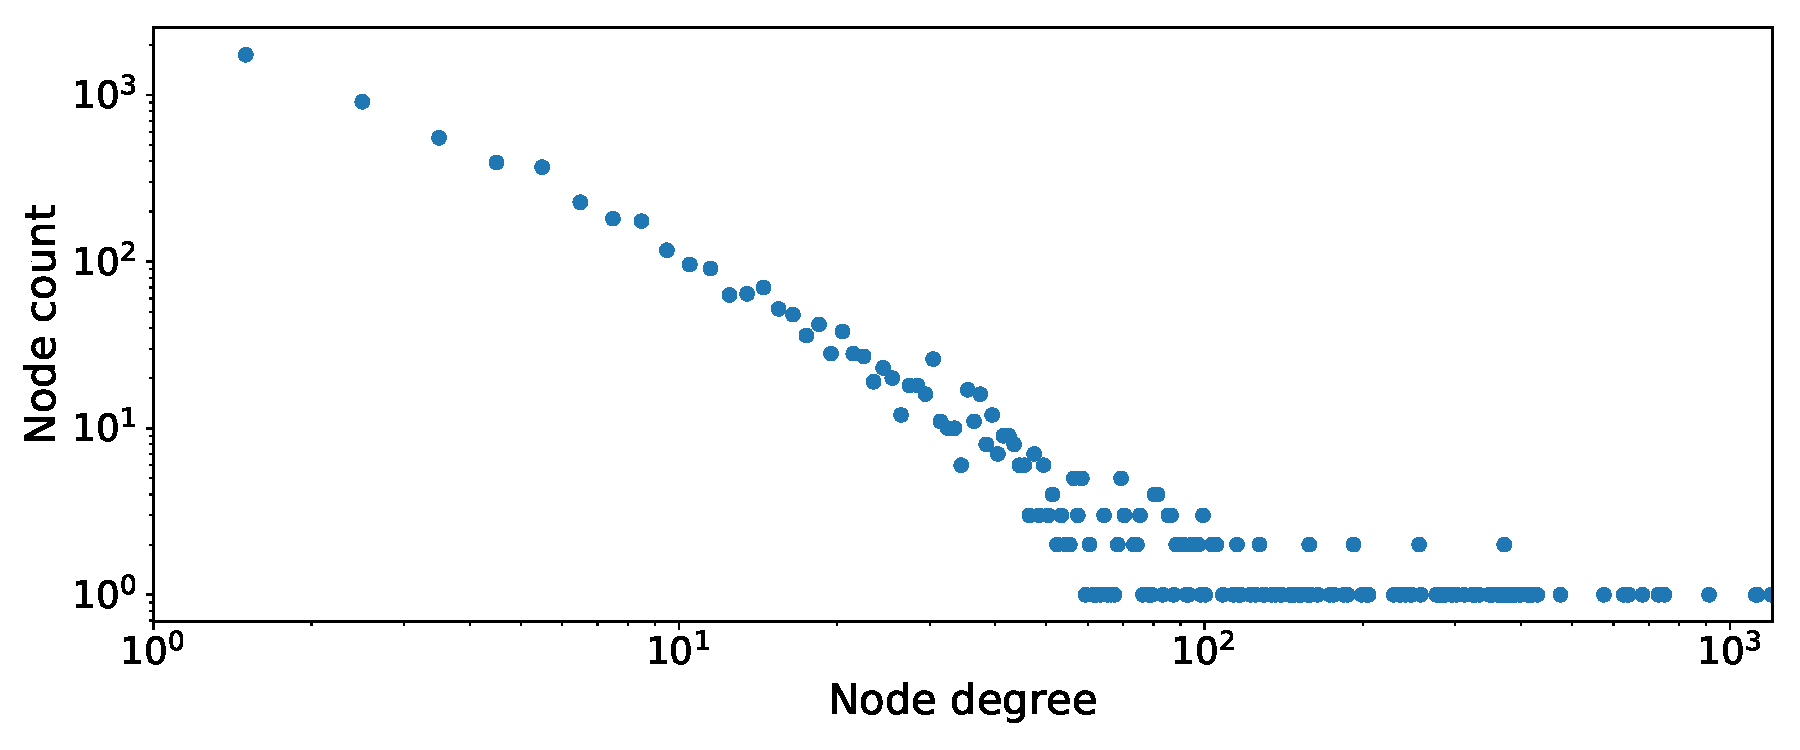
\includegraphics[width=\columnwidth]{node-degree-histogram}
	\caption{Node degree distribution.\label{fig:node-degree-histogram}}
\end{figure}

\begin{figure}[tb]
	\centering
	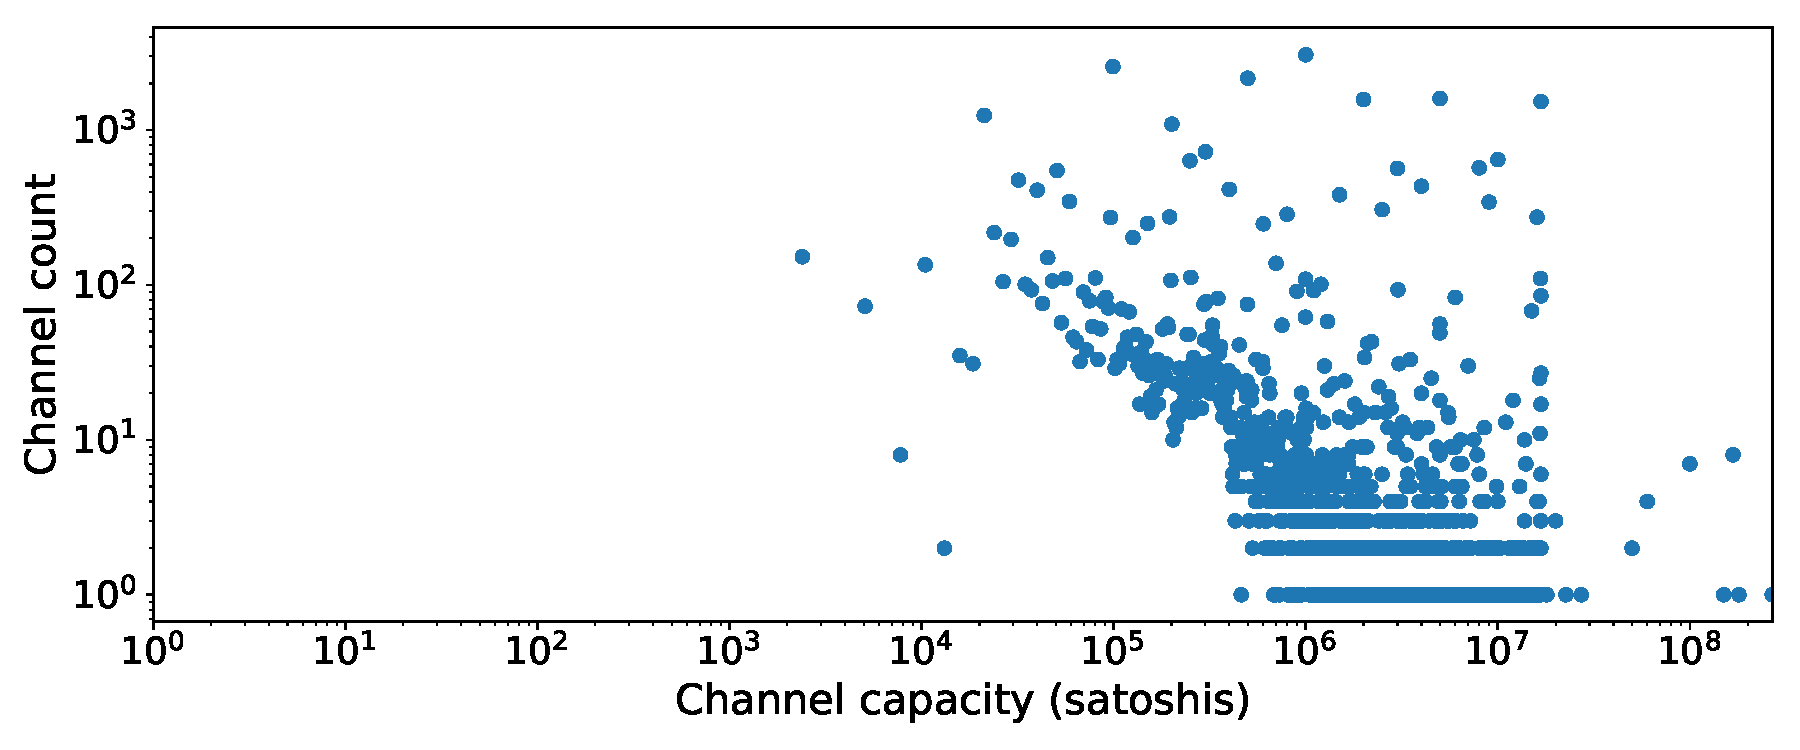
\includegraphics[width=\columnwidth]{channel-capacity-histogram}
	\caption{Channel capacity distribution.\label{fig:channel-capacity-histogram}}
\end{figure}

\subsubsection*{Ethical considerations} 
Our analysis is based solely on publicly available data. 
We do not interfere with the LN activity, nor deanonymize any of its nodes. 


\section{Security and privacy: theory and practice}
\label{sec:sec-priv-attacks}

As introduced in~\cref{sec:background}, the LN builds upon Hash Time-Lock Contracts aiming to achieve 
atomicity in multi-hop payments.
However,~\cite{Malavolta2019} argues that due to the \emph{wormhole attack} atomicity does not hold in LN.
Another LN study~\cite{Malavolta2017} shows that privacy of LN users and their transactions can be breached.
While the aforementioned works demonstrate the feasibility of these attacks, 
their effectiveness in practice depends, among other factors, on the topology of the LN.
In this experiment, we aim to identify the impact of these security and privacy issues in our snapshot of the LN.
%We study the prevalence of three attacks: the wormhole attack, value privacy, and relationship anonymity.
%We first describe our methodology, and then present the results for the three attacks along with the necessary background.

\subsection{Security and privacy attacks: background}

\begin{figure*}[tb]
	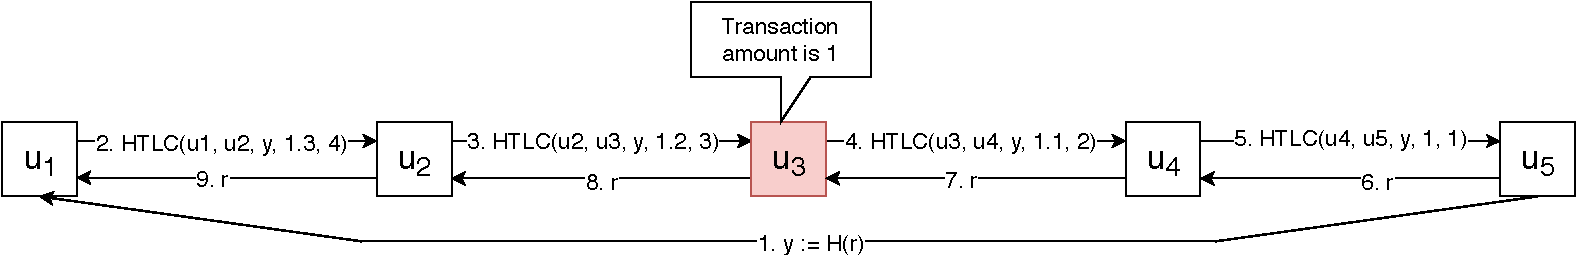
\includegraphics[width=\textwidth]{vp-figure.pdf}
	
	\vspace{0.3cm}
	
	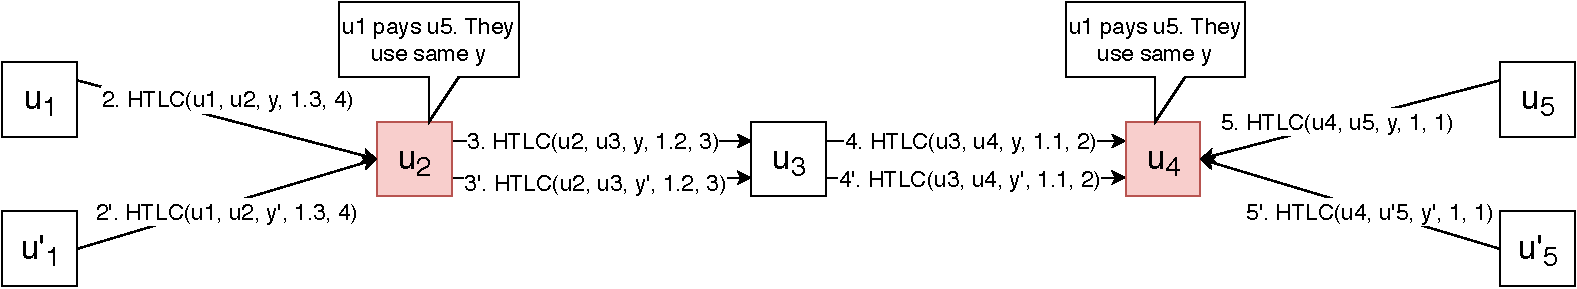
\includegraphics[width=\textwidth]{ra-figure.pdf}
	
	\vspace{0.3cm}
	
	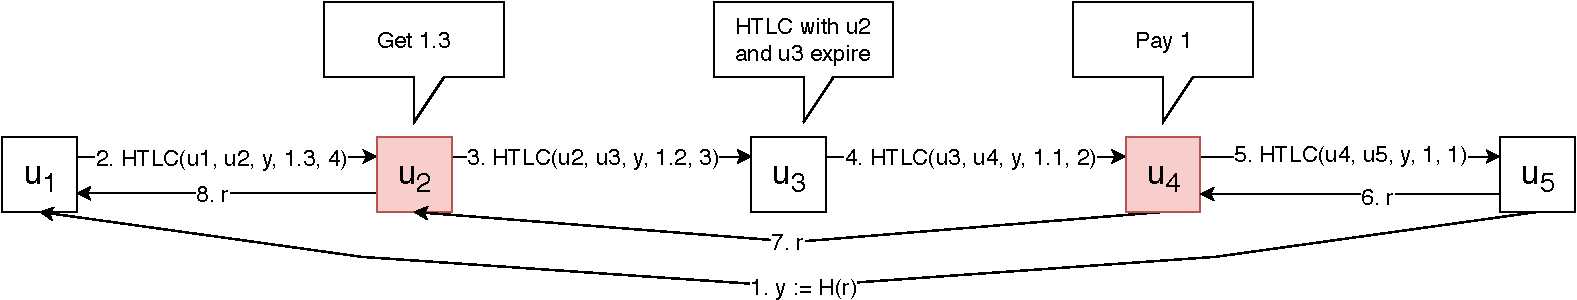
\includegraphics[width=\textwidth]{wa-figure.pdf}
	
	\caption{\label{fig:wormhole-attack} An illustrative example of value privacy (top), relationship anonymity (middle), and the wormhole attack (bottom).}
\end{figure*}

\subsubsection{Value privacy~\cite{Malavolta2017}}
Intuitively, value privacy ensures that for a transaction involving only honest users, 
corrupted users outside of the path learn no information about the transaction value.
This notion thus heavily relies on the existence of paths without adversarial nodes.  
Otherwise, an adversarial intermediary node can trivially learn the (upper bound of the) amount of a transaction that it forwards. 
For instance, in~\cref{fig:wormhole-attack} the adversary $u_3$
forwards $1.2$ coins to $u_4$, estimating the transaction amount at around $1$ coin plus forwarding fees.

\subsubsection{Relationship anonymity~\cite{Malavolta2017}}
Intuitively, relationship anonymity ensures that given two simultaneous transactions 
between two pairs of nodes $(u_1, u_2)$ and $(u'_1, u'_2)$ routed through the same path of intermediary 
users $i_1, \ldots, i_n$, the adversary controlling some of those intermediaries cannot tell who is paying to whom with probability better than $1/2$.
However, this is not achieved in the LN.
An adversary controlling $i_1$ and $i_n$ can use the cryptographic challenge included in the HTLC to 
determine who pays to whom.
For instance, in~\cref{fig:wormhole-attack} the adversary controlling $u_2$ 
and $u_4$ can determine that $u_1$ is transacting with $u_5$ as the same value $y$ is used along the whole path. 
Similarly, $u_2$ and $u_4$ can determine that $u'_1$ is transacting with $u'_5$ as the same $y'$ is being used along the path. 

\subsubsection{The wormhole attack~\cite{Malavolta2019}}
In the wormhole attack, two colluding nodes in a transaction path prevent honest intermediaries from 
participating in the successful completion of the payment, stealing the 
fees initially intended for honest intermediaries.\footnote{One may argue that this is not an attack, as from the sender's point of view the payment is delivered. Yet, this attack takes the economic incentive that honest users have to forward payments in the first place.} 
%On top of that, coins are locked in the HTLCs with honest 
%intermediaries longer than required for a successful transaction, thereby preventing honest users from 
%participating in other (possibly successful) transactions. 
An example of the wormhole attack is depicted in~\cref{fig:wormhole-attack}. 
Here, $u_4$ does not send the opening value $r$ to $u_3$ (step 7 in~\cref{fig:htlc}) to fulfill the HTLC previously set in this channel. 
Instead, $u_4$ sends the value $r$ to $u_2$ outside of the LN protocol, which allows $u_2$ to settle the HTLC with $u_1$. 
As a consequence, contracts with $u_3$ expire, simulating transaction failure and
preventing $u_3$ from participating in the successful completion of the transaction. 



\subsection{Methodology}
In this section, we describe how we study the proneness of the LN to attacks with respect to the value privacy, relationship anonymity, and wormhole attack scenarios. 

We first compute the paths between pairs of nodes.
Given a pair of nodes $u_1$ and $u_2$, 
we compute the list of paths that connect them with one restriction:
we consider only the paths with at most three intermediary nodes.
We observe that paths of this length suffice to allow more than $85\%$ of 
transactions between a random pair of nodes (\cref{fig:payment-success}).
% for transactions amounts expected in the LN \missing{add citation here}.
%We restrict our experiment to paths of this length because of high computational requirements 
%caused by significantly higher number of paths for higher length limit.
%Due to high computational requirements, we run a smaller number of randomized experiments for the higher path length limit.
%We remark that in the Lightning Network shorter paths are more likely to be chosen due to lower fees and higher probability of payment success.
We also note that these paths allow us to exemplify all attacks that we want to study in this experiment.
\begin{figure}
	\centering
	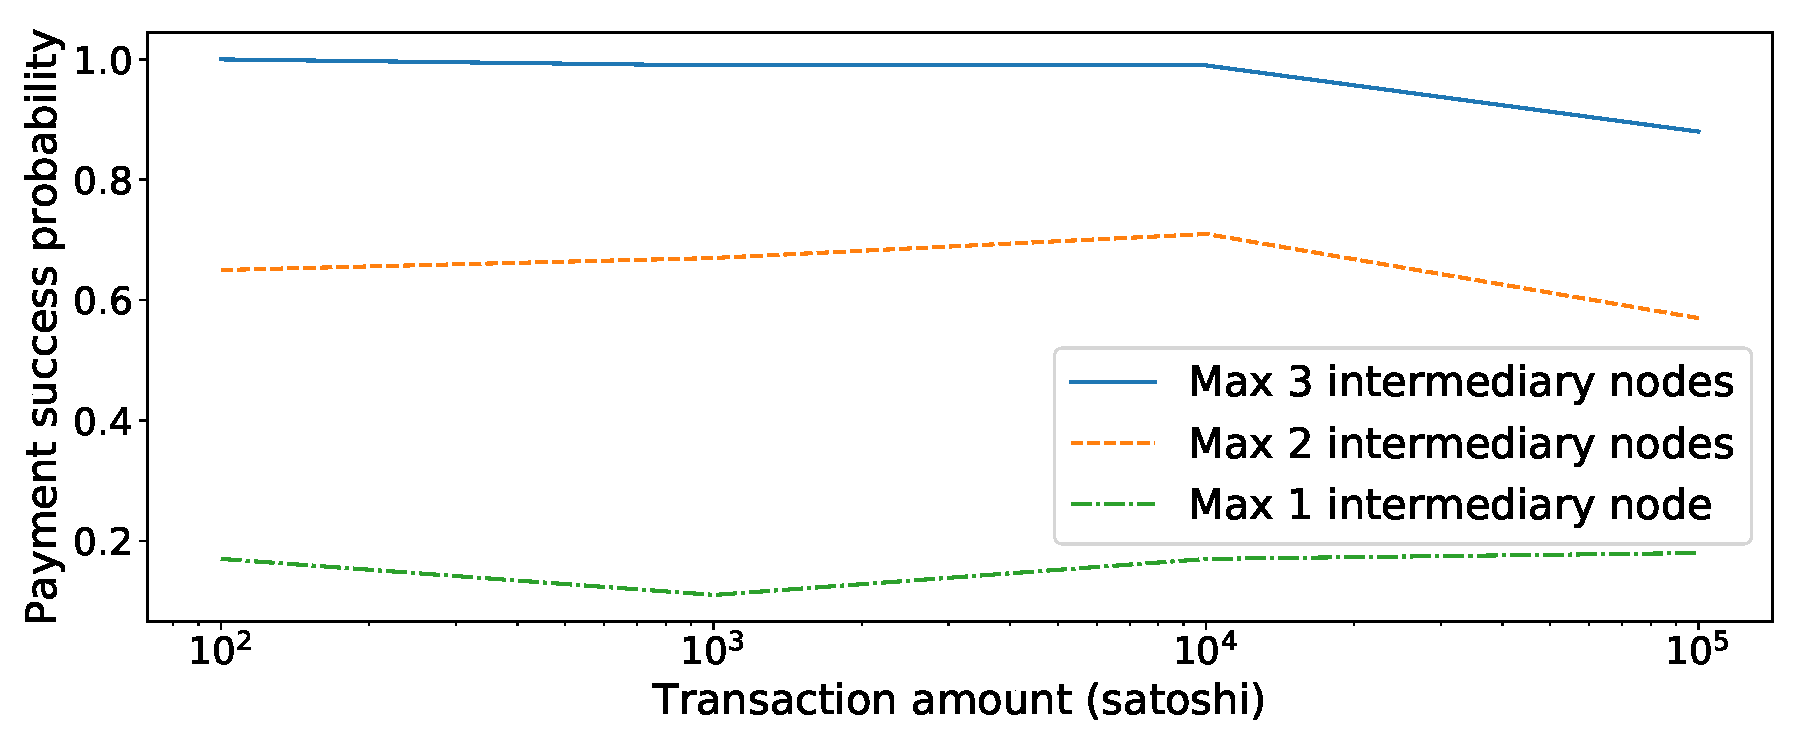
\includegraphics[width=\columnwidth]{payment-success}
	\caption{The share of experiment runs where paths with sufficient capacity exist between sender and receiver.}
	\label{fig:payment-success}
\end{figure}

%We also note that while LN protocol limits the length of paths at 20~hops, LN clients don't have to find all paths of lengths lower than the limit.
%Instead, they iterate through possible paths until the payment succeeds.

%We check the effectiveness of the wormhole attack by randomly selecting a representative sample of the population 
%of LN nodes composed of 1000~pairs of nodes.
%We set a payment amount $x$ for the experiment to one of the values: $10^2$, $10^3$, $10^4$, $10^5$ satoshis.
%For each pair of nodes ($u_1, u_2$), we obtain all possible paths connecting them that contain at most 
%five nodes (i.e., $u_1$, $u_2$ and up to three intermediary nodes).
%We restrict our experiment to paths of this length because of high computational requirements caused by significantly higher number of paths for higher length limit.
%The average number of paths between two random nodes is 24 with up to 4 nodes is 24, 3550~with up to 5 nodes, and approximately 200~thousand for up to 6 nodes.
%We limit our experiments to paths with at most 5~nodes, as this allows us to exemplify all attacks including the wormhole attack.
%Moreover, in the majority of cases the nodes would have paths shorter than 5~nodes (see below), and in the real network shorter paths are more likely to be chosen due to lower fees and lower chances of payment failure.
%Approx time for one experiment with 1000 iterations: 3 hops: tens of minutes, 4: ~4 hours, 5: ~days.

%We only consider $u_1$ with have a channel with the capacity not less than $x$.
%The rationale behind this restriction is the following.
%We aim to estimate the probability that a payment will traverse through a vulnerable path.
%When calculating routes, the sender only takes into account only the local channels with sufficient capacity.
%If there are no such channels, the payment is impossible regardless of the network structure.

Let $\textit{paths}_{\langle u_1, u_2 \rangle}$ be the set of paths between $u_1$ and $u_2$ thereby computed. 
We further prune the set $\textit{paths}_{\langle u_1, u_2 \rangle}$ into a subset 
$\textit{paths}_{\langle u_1, u_2 \rangle, x}$, containing  only the paths that 
allow to transfer at least $x$ satoshis. 
For instance, $\textit{paths}_{\langle u_1, u_2 \rangle, 10}$ 
contains the paths between $u_1$ and $u_2$ allowing to transfer at least $10$ satoshis. 


For a channel to be capable of transferring $x$ satoshis from $u_i$ to $u_j$, $u_i$ must have a balance of 
at least $x$ satoshis. However, the current balance of each counterparty in a channel is not publicly available. 
Thus, we consider a path suitable for a given transaction if the total capacity of every channel 
in the path is not lower than the transaction amount, independently of how this capacity 
is distributed among the two channel counterparties. 
This heuristic might consider a path suitable for a transaction while it is not.
We nevertheless follow this heuristic as it is also used by LN nodes in practice. 
%, which leads to payments trying multiple paths before succeeding.
% \missing{add reason why it is still ok to consider this heuristic - do we have other choice?}

%We estimate the share of cases when at least one suitable path exists for various values of $x$.
% results-1571154370.json (with has_path function)
%We arrive at the following shares of payments with at least one suitable path: 99.3, 99.2, 99.0, and 86.6 percent for 100, 1k, 10k, and 100k satoshis, respectively.
%The results indicate that while it is possible to find a path for smaller payments in the majority of cases, the Lightning network can not yet reliably support larger payments.\footnote{100k satoshis are equivalent to 100~USD at 10k USD per bitcoin.}
%The most likely explanation of the drop in success rate is the lack of incoming capacity at the receiver's side (see Section~\ref{sec:liquidity} for the measurement of liquidity -- a related metric).

%For each attack, we present the definition of a path prone to this attack.
%We consider all other paths safe.

As the next step, we study the effectiveness of the selected attack.
For a chosen transaction amount $x$,
we split the set $\textit{paths}_{\langle u_1, u_2 \rangle, x}$ into two subsets:
(i) $\textit{paths-prone}_{\langle u_1, u_2 \rangle, x}$: The subset of paths that are prone to the attack;
(ii) $\textit{paths-safe}_{\langle u_1, u_2 \rangle, x}$:  The subset of paths that are not susceptible to being attacked. 
The definition of a path of the form $u_1 \rightarrow i_1 \rightarrow  \ldots \rightarrow i_n \rightarrow u_2$  being 
prone to the attack depends on the type of the attack:
\begin{itemize}
	
	\item \textit{Value privacy:} We say that a path is prone to the 
	value privacy attack if any of the intermediary nodes is under adversarial control. 
	
	\item \textit{Relationship anonymity:} We say that a path  
	is prone to the relationship anonymity attack if nodes $i_1$ and $i_n$ are under adversarial control.
	
	\item \textit{Wormhole attack:} We say that a path  
	is prone to the wormhole attack if there exist two non-neighboring intermediary 
	nodes $i_j$ and $i_k$ that are under adversarial control (i.e., $j < k$ and $k \neq j + 1$). 
	
\end{itemize}

%We remark that there exist two differences in the definitions of a prone path in the wormhole attack and the relationship anonymity attack. 
%First, for the relationship anonymity attack we do not require that there is an honest user between the two adversarial nodes.
%For instance, a path of the form $u_1 \rightarrow i_1 \rightarrow i_2 \rightarrow u_2$ where $i_1$ and $i_2$ are under adversarial control,  would be considered prone to the relationship anonymity attack but safe against the wormhole attack. 
%Second, for the relationship anonymity attack we require that the adversary controls the nodes neighboring the sender and the receiver. For instance, 
%a path of the form $u_1 \rightarrow i_1 \rightarrow i_2 \rightarrow i_3 \rightarrow i_4 \rightarrow u_2$ where $i_2$ and $i_4$ are under adversarial control, would be prone to the wormhole attack but safe against the relationship anonymity attack. 

We remark that there exist a difference in the definition of a prone path in the wormhole attack and the relationship anonymity attack. 
For the relationship anonymity attack we do not require that there is an honest user between the two adversarial nodes.
For instance, a path of the form $u_1 \rightarrow i_1 \rightarrow i_2 \rightarrow u_2$ where $i_1$ and $i_2$ are under adversarial control,  would be considered prone to the relationship anonymity attack but safe against the wormhole attack. 

Another aspect that we consider is which nodes are under adversarial control.
We follow three strategies. 
First, we assume that nodes with highest degree (i.e.,~highly connected nodes) are colluding to carry out an attack. 
Highly connected nodes are interesting to study as they are the ones with the highest stake in the network. 
Thus, an adversary might attempt to corrupt them (e.g.,~by bribery or stealing the private key) to maximize the effect of the attack. 
%whereas it requires significant efforts as highly connected nodes are expected to be run by technically knowledgeable individuals.
Second, we assume that nodes with the highest total capacity in their adjacent channels are corrupted.
Finally, we consider that random nodes in the network are colluding to carry out an attack. 
We model here that any node (independently of its node degree) might be corrupted.
For instance, the same user might create several LN nodes and place them at strategic positions in the LN to carry out the attacks we study here. 

We refine our aforementioned path datasets to consider these three attacks strategies.
In particular, for each number of malicious nodes ($y$) and each strategy, we re-split the set $\textit{paths-prone}_{\langle u_1, u_2 \rangle, x}$ 
between those prone to the attack and those otherwise safe. 
%We thus split the paths as aforementioned several times, considering each time that a different number of highly connected nodes are malicious.
For instance, we denote by $\textit{paths-prone}_{\langle u_1, u_2 \rangle, x, y\textit{-con}}$ 
the subset of paths between 
$u_1$ and $u_2$ that allow to transfer $x$ satoshis and that are prone 
to the attack if $y$ nodes with the highest node degree are corrupted. 
Correspondingly, we denote by $\textit{paths-prone}_{\langle u_1, u_2 \rangle, x, y\textit{-ran}}$ 
the subset of paths between 
$u_1$ and $u_2$ that allow to transfer $x$ satoshis and that are prone 
to the attack if $y$ nodes chosen uniformly at random are corrupted. 

Finally, for each attack strategy, we consider $$\alpha_{\langle u_i, u_j \rangle} := \frac{|\textit{paths-prone}_{\langle u_i, u_j \rangle, x, y}|}{|\textit{paths-prone}_{\langle u_i, u_j \rangle, x, y}| + |\textit{paths-safe}_{\langle u_i, u_j \rangle, x, y}|}$$ 
the probability that a transaction between $u_i$ and $u_j$ is vulnerable to the attack. 
Averaging across all the pairs of nodes tested, we extract the final probabilities reported in~\cref{fig:fig-all-attacks}.


\subsection{Results and discussion}

In this section, we present the results shown in~\cref{fig:fig-all-attacks} and discuss their implications. 
\begin{figure*}
	\centering
	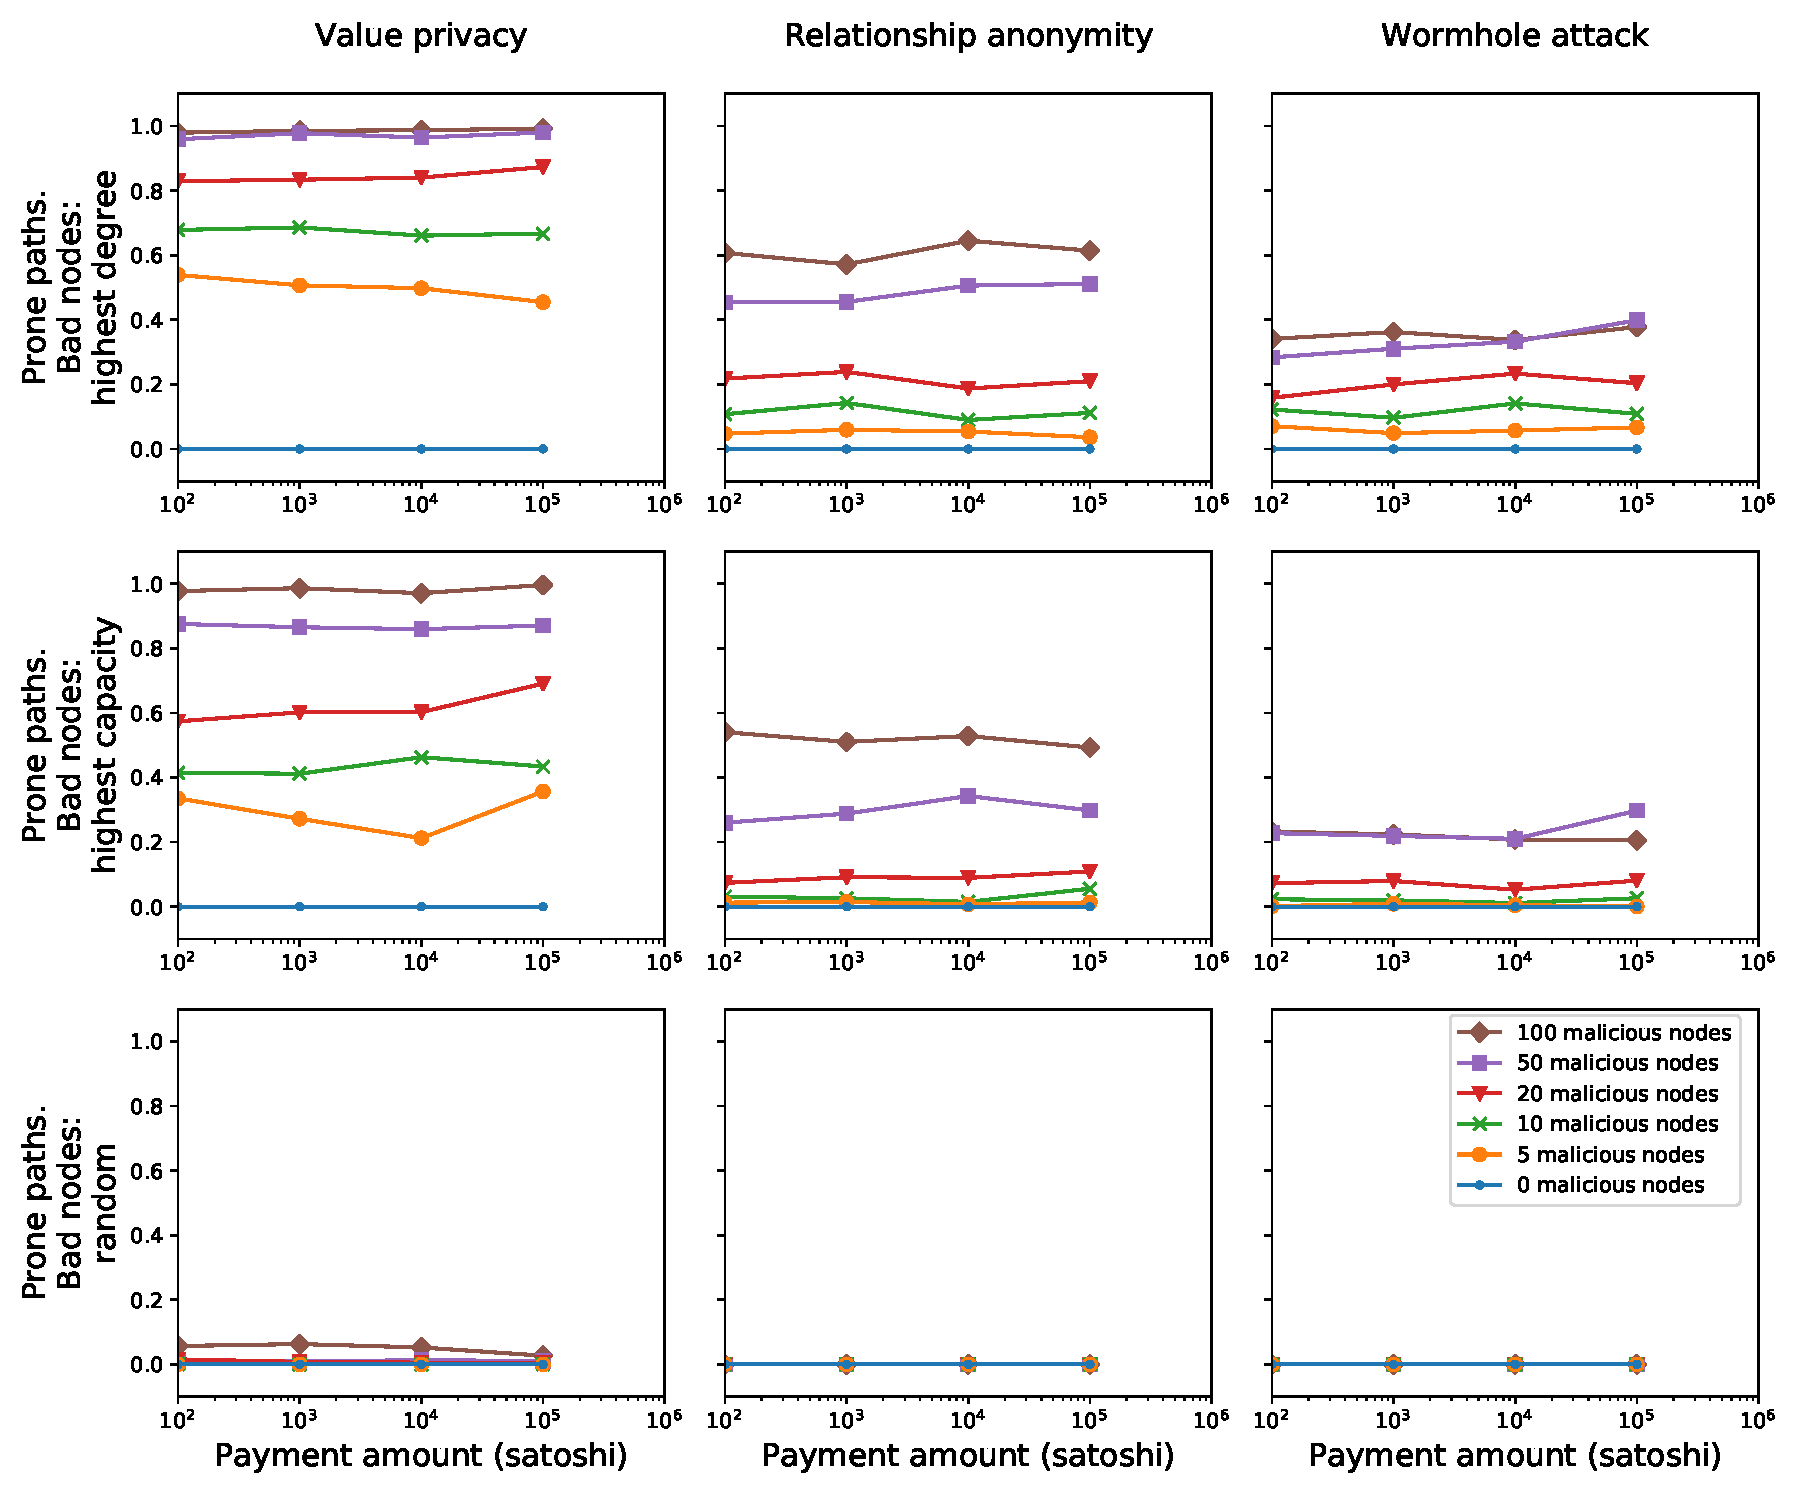
\includegraphics[width=\textwidth]{fig-all-attacks}
	\caption{Share of vulnerable paths for each attack, considering that highest degree nodes are compromised (top), highest capacity nodes are compromised (middle), or random nodes are compromised (bottom).}
	\label{fig:fig-all-attacks}
\end{figure*}

For every attack and a given number of compromised nodes, the share of prone paths is relatively stable for all payment amounts.
This indicates that the payment amount does not significantly affect the security of payments.
% (though it affects the probability of its success as shown in~\cref{fig:payment-success}).

The three attacks differ in how quickly the share of prone paths changes as the number of compromised nodes increases.
For value privacy, the effect of additional highly-connected nodes being compromised is the most profound: 
the share of prone paths is $50\%$ if only the $5$ most connected nodes are compromised 
and nearly $100\%$ if the $100$ most connected nodes are compromised. 
We conclude thus that an adversary needs to corrupt only $2\%$ of the nodes to (almost) completely nullify any value privacy guarantee in the LN.

We observe that the average share of prone paths decreases for relationship anonymity.
Yet, the adversary controlling the $100$ most connected nodes can launch the relationship anonymity attack on about $70\%$ of the paths. 
Interestingly, the adversary has fewer possibilities to launch the wormhole attack.
For instance, even with $100$ most connected nodes corrupted, around $30\%$ of the paths are prone to the attack.
While this is still a crucial security issue, this reduction in the effectiveness of the attack 
may be explained by the fact that the wormhole attack is the most restrictive on path structure, and thus it 
has the lowest share of vulnerable paths. 
%For relationship anonymity, path safety is less sensitive to the increase in the number of compromised nodes: around 90\% and 30\% of paths are safe with 5~and 100~compromised nodes, respectively.

%Finally, the wormhole attack is the least affected, with 90\% and 30\% of safe paths with 5~and 100~compromised nodes.
%This may be explained by the fact that the structure of paths prone to value privacy attack is simpler (one malicious node must be at any point in the path), therefore there are more prone paths.
%Relationship anonymity requires a more elaborate structure (the first and the last nodes are malicious), and there are fewer such paths.
%Finally, wormhole attack is the most restrictive on path structure, and has the lowest share of vulnerable paths.
Increasing the number of compromised nodes results in fewer vulnerable paths if compromised nodes are those with the channels holding the highest capacity, as opposed to highest degree nodes.
This distinction is most profound for relationship anonymity, e.g.,~there are around $50\%$~for $50$~highest degree corrupted nodes, but only around $25\%$~vulnerable paths for $50$~highest capacity corrupted nodes.
%For a roting node to attract payments, good connectivity is more important than high capacity.
This may be explained by the fact that routing algorithms optimize for low path length.
Note that capacity of forwarding channels is not as important as good connectivity, especially for payments of small and medium amounts.

Finally, we consider random nodes compromised instead of the most connected nodes.
%This experiment acts as a baseline for the attack efficiency in the case when the adversary does not have the means to take over professionally maintained nodes.
In contrast to the previous results, we observe that less than $10\%$ of paths are prone to value privacy and nearly no path is prone 
to relationship anonymity and wormhole attack.
We conjecture that this is because randomly selected nodes have few connections (note the degree distribution in Figure~\ref{fig:node-degree-histogram}), and thus their compromise does not affect routing at large.
%Therefore, it is beneficial for an adversary to target highly connected nodes, as this substantially increases the impact of the attack.

%\todo[inline]{@Sergey: Let's have only one path length. It is confusing and hard to parse otherwise.}
%We also perform the same experiments considering longer paths of up to 4 intermediary nodes.
%Due to high computational requirements of the path finding function, we only perform the experiments for 2~amounts (1000 and 100000~satoshis), and 8~iterations.
%The experiments indicate that the increase in the path length by one hop does not significantly affect the results outlined above.

In summary, 
the results of this experiment show that highly connected nodes and nodes with high capacity links have a high impact on the security and privacy of the LN.
Assuming that paths are selected uniformly at random from the set of available paths, 
an adversary that selectively corrupts $100$ (i.e.,~only $2\%$) 
of LN nodes can effectively learn all the transaction values, 
the sender and the receiver for the vast majority of transactions, 
as well as carry out the wormhole attack in about $30\%$ of the paths. 
This shows that the security and privacy attacks shown in theory are indeed crucial in practice. 

Carrying out such an attack might not be infeasible in the live network. We 
note that a large number of highly connected LN nodes is controlled by an unknown entity under the pseudonym LNBIG.
It controls 23~out of top~50 highest connected nodes~\cite{1MLTopConnected} and $40\%$ of the network capacity~\cite{TheBlockLNBIG}.
%This means that a large-scale privacy attack on LN may be performed by compromising LNBIG alone.
%The attacks can further be amplified by using part of LNBIG's capacity to temporarily block other hubs and force more payments to be routed through the compromised nodes.

\subsection{Countermeasures}
We assume in our study that every two nodes carry out their transactions  
along a subset of paths chosen uniformly at random from the set of all available paths between them. 
However, LN nodes might implement different routing strategies. 
%In particular, nodes joining the LN should carefully choose their channel counterparties. 
For instance, while routing through well-connected nodes improves the chances to reach the receiver through a short, highly liquid path, 
the sender might connect to low degree nodes.
This would make the node degree distribution more even at the cost of connectivity and reduce the probability of choosing paths prone to the 
attacks studied in this experiment. 
We envision thus that there is a tradeoff between connectivity on the one hand and security and privacy on the other,
which constitutes a venue for future work.
A node may also route transactions through a trusted proxy node, 
thus guaranteeing that the first node in a path is not compromised.
This would mitigate the relationship anonymity and wormhole attacks (if the total path length is bounded to contain at most three intermediaries).
As the LN protocol is still evolving, the results of the experiments presented in this section should be considered 
for the next design decisions.

Routing protocols for the LN is an active research area~\cite{Roos2018, Sivaraman2018, Malavolta2017a, Prihodko2016, Grunspan2018, Bagaria2019, Osuntokun2018, Pickhardt2019, ZmnSCPxj2019, ZmnSCPxj2019a, ZmnSCPxj2019b}.
The results of our experiments suggest that, although largely omitted so far, 
the security and privacy attacks here studied are a crucial variable to consider when designing routing protocols. 


\section{HTLC limit in the Lightning Network}
\label{sec:attack}

In this section, we describe a limitation in the LN design 
stemming from the way it manages concurrent payments. 
A payment channel, even with sufficient capacity, can hold only 
a certain number of concurrent payments (governed by HTLCs), leading to capacity under-utilization. 
%While concurrent payments are theoretically 
%limited by the capacity (i.e., number of satohsis) in the channel, in practice 
%they are limited to a lower number that leads to capacity under-utilization. 
We study the effect of this limitation.
First, we evaluate how the number of concurrent payments in LN 
is majoritarily bounded by the number of concurrent HTLCs allowed at each channel. 
Second, we show how a malicious node can abuse this 
limitation to isolate parts of the network, 
which ultimately results in a network-wide DoS attack.
We provide estimates for the cost of such an attack, showing that it is within range for a moderately resourceful attacker. 
We finally discuss potential countermeasures.

\subsection{Background} \label{max-htlc-background}

Among other transaction validity rules, a Bitcoin transaction must be smaller than 100~KB (transaction size limit\cite{StandardTxBitcoinSE, BitcoinCoreMaxTxWeight}).\footnote{Bitcoin~Core, the reference Bitcoin implementation, defines a \textit{standard} transaction. Transaction size limit is a part of this definition. While non-standard transactions may be valid according to the consensus rules, Bitcoin~Core nodes do not propagate them. As Bitcoin~Core nodes constitute $97\%$ of the network~\cite{CoinDance}, non-standard transactions are highly unlikely to get confirmed.}
An LN channel can not contain more than 966~unsettled HTLCs, as prescribed in~\cite{BOLT2Rationale}.
This limit ensures that both counterparties can close the channel using one valid Bitcoin transaction.\footnote{The specification also points out that this limit ensures that the related messages conform to the limitation of the LN protocol, which limits the size of a message to $65535$~bytes.}
Hereby we refer to the limitation described above as the \textit{HTLC limit}.

Despite the perceived focus on micropayments, LN does not fully support transactions of very small value.
Every HTLC makes the potential closing transaction larger, and the on-chain fees higher.
Redeeming very small outputs on-chain can be more expensive than their value.
Therefore BOLT specifications prescribe that nodes negotiate the \textit{dust limit} before opening a channel, and for payments below this limit, no HTLCs are created (see \textit{trimmed HTLCs}~\cite{BOLT3Trimmed}).
%They are added to on-chain fees in case the channel closes at the current state.
Out of the three most popular LN implementations, c-lightning and Eclair use the default dust limit of $546$~satoshis.
LND estimates the dust limit dynamically.
We thus hereby assume $546$~satoshis as the dust limit.


%This effectively restricts the amount of information that a transaction can contain.

\subsection{Estimating the HTLC limit effect on LN scalability}	\label{estimating-concurrent channel updates}

In this section, we estimate the effect of the HTLC limit on the number of concurrent channel updates.
%In particular, we calculate an upper bound of the number of concurrent channel updates with and without the HTLC limit.
%We derive thereby the effect of the HTLC limit on the LN performance.

%\paragraph{Concurrent channel updates}
%Consider a channel with a capacity $c$.
%Given a transaction amount $a$, this channel can perform $c / a$ updates concurrently.
%However, given the HTLC limit, the number of concurrent updates is at most 966 (483 in each direction).

%We estimate the effect of the HTLC limit on the network performance by comparing the network-wide limit on the number of concurrent updates without the limit, i.e.,~based on the capacity alone ($u_{cap}$), and with the HTLC limit ($u_{HTLC}$).

Let $D$ be the dust limit.
We only consider amounts higher than $D$.
Let $C$ be the total network capacity (i.e., the sum of the individual capacities of all channels).
Let $a_\textit{avg}$ be the average transaction amount. 
Then, we say that the limit on concurrent updates based solely on capacity is defined as   
$u_\textit{cap} := C / a_\textit{avg}$.
In contrast, the limit on concurrent updates 
considering the HTLC limit is $u_\textit{HTLC} = N * 966$.
where $N$ is the number of channels. We remark here that $u_\textit{HTLC}$ does not depend on transaction amounts.

Given those two values, we define the 
\textit{effective update rate} $ur_\textit{eff}$ as the ratio between the actual limit on concurrent 
transactions when considering the HTLC limit and the theoretical 
limit based solely on capacity:

\[ur_\textit{eff} = \frac{min(u_\textit{cap}, u_\textit{HTLC})}{u_\textit{cap}}\]

Note that the effective update rate $ur_\textit{eff}$ depends on 
the average transaction amount, as shown in Figure~\ref{fig:effective-channel-updates}.
%For very low amounts, the effective number of concurrent updates is at the theoretical maximum.
Starting from $D$, there is a gap between the effective number of concurrent updates and what could be theoretically possible in the absence of the HTLC limit. 
%For instance, $ur_\textit{eff} = 37.43\%$ for $1000$~satoshis ($0.08$~USD) and $3.81\%$ for $100$~satoshis ($0.008$~USD).
We observe that $2677$ satoshis ($0.24$~USD) is the \textit{borderline amount}: for higher average transaction amounts, 
the limiting factor for the number of concurrent channel updates is channel capacity.
For amounts between $D$ and $2677$ satoshis, the limiting factor is the HTLC limit.
%For transactions with higher value than $2677$~satoshis LN is limited by capacity, 
%and for transactions of lower value the restriction on the number of in-flight HTLCs is the limiting factor.

\begin{figure}
	\centering
	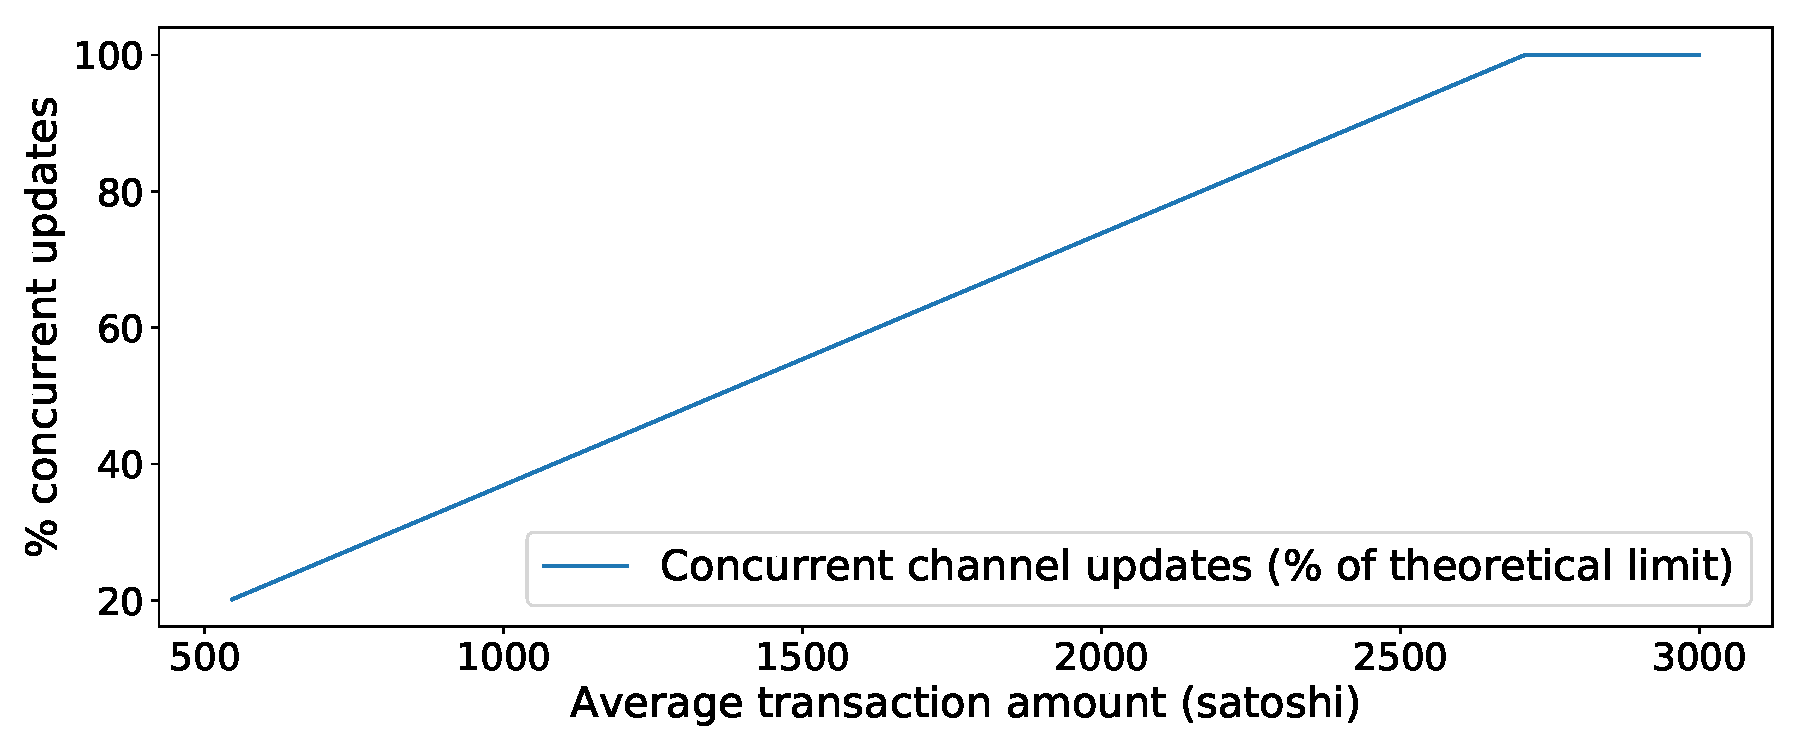
\includegraphics[width=\columnwidth]{effective-channel-updates}
	\caption{Ratio between the current limit on concurrent channel updates and the theoretically possible 
	capacity-based limit.\label{fig:effective-channel-updates}}
\end{figure}

\subsubsection*{Affected channels}
The $ur_\textit{eff}$ is an aggregated measurement that does not shed 
light on how the issue affects individual channels.  
Given that, we now study how many channels are affected by the HTLC limit.
The number of affected channels depends on the average transaction amount $a_\textit{avg}$. 
For high values of $a_\textit{avg}$, it is more likely that 
the effective update rate of a channel is limited by its capacity, 
whereas the HTLC limit would determine the update rate cap for small values of $a_\textit{avg}$.
We quantify this as follows.
Given a fixed average transaction amount $a_\textit{avg}$, 
we consider a channel \textit{affected} by the HTLC limit if $u_{\textit{HTLC},a_\textit{avg}} < u_{\textit{cap},a_\textit{avg}}$, i.e, $u_{\textit{eff},a_\textit{avg}} < 100\%$ (\cref{fig:affected-channels}).
%Note that contrary to network-wide calculations in the previous paragraph, here we consider the capacity of each channel individually.
%As in~\cref{fig:effective-channel-updates}, amounts lower than the dust limit have no effect on the network's throughput.
%$88.0\%$ of channels are affected with $a_\textit{avg}=100$, and $44.72\%$ are affected for $a_\textit{avg}=1000$.
%Drops on the graph correspond to popular channel capacities (?).

\begin{figure}
	\centering
	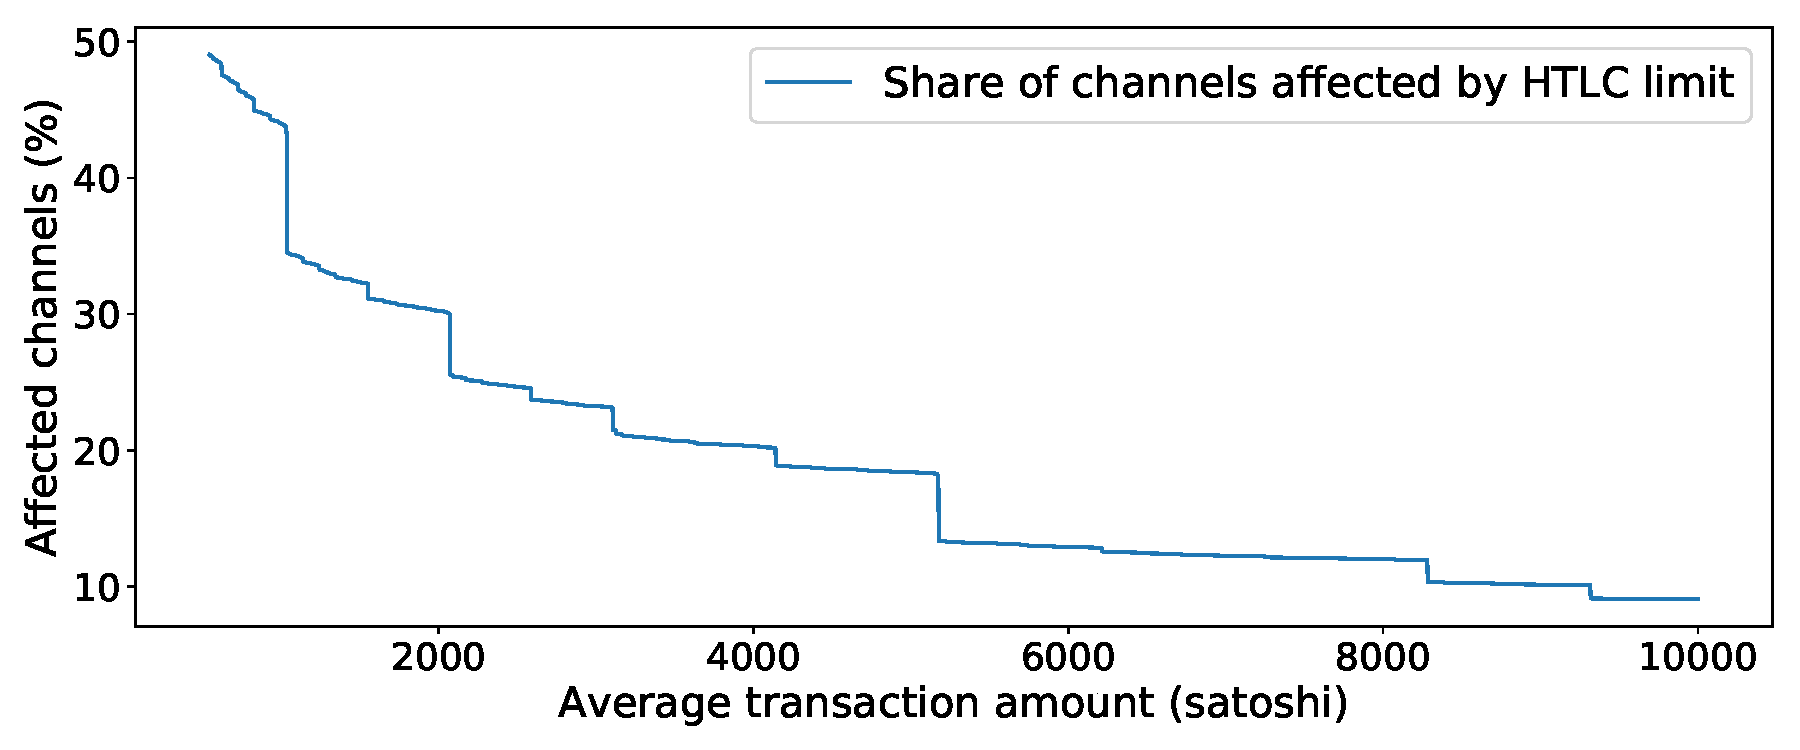
\includegraphics[width=\columnwidth]{affected-channels}
	\caption{Share of channels affected by the HTLC limit for different transaction amounts. \label{fig:affected-channels}}
\end{figure}



\subsubsection*{The effect of the HTLC limit over time}

%We use the set of historic snapshots (LNHist) to study how LN throughput changed over time.
%The dynamics regarding TPS limits shoes that the network throughput continues to grow with the increasing capacity and the number of channels.
%However, not enough channels (hence, HTLC slots) are being added to LN to accommodate the growing capacity.
%Therefore, LN performance is being held back by the HTLC limit for even smaller amount, as seen on Figure~\ref{fig:historic-tps}.
%\begin{figure}
%	\centering
%	\includegraphics[width=\columnwidth]{figures/historic-tps}
%	\caption{Historic TPS limits.\label{fig:historic-tps}}
%\end{figure}

We study the effect of the HTLC limit on the LN using our historical snapshots \emph{LNHist}.
For each monthly snapshot and four assumed average transaction amounts, we calculate the share of channels affected by the HTLC limit (\cref{fig:historic-htlc-limited-share}).
As expected, the HTLC limit becomes a more pressing issue 
with smaller transaction amounts, if they are higher than the dust limit.
We also observe that the share of affected channels has been increasing in the early months of LN and has remained stable since mid-2019.

We finally study how the \textit{borderline amount} has changed over time. 
%-- the average transaction amount for which the restriction on concurrent payments imposed by channel capacities is equal to the HTLC limit -- 
As~\cref{fig:historic-borderline-amount} shows, the HTLC limit finds 
its inflexion point in transaction amount at approximately $2500$~satoshis, with the borderline amount stabilizing in mid-2019, after the initial growth.

\begin{figure}[tb]
	\centering
	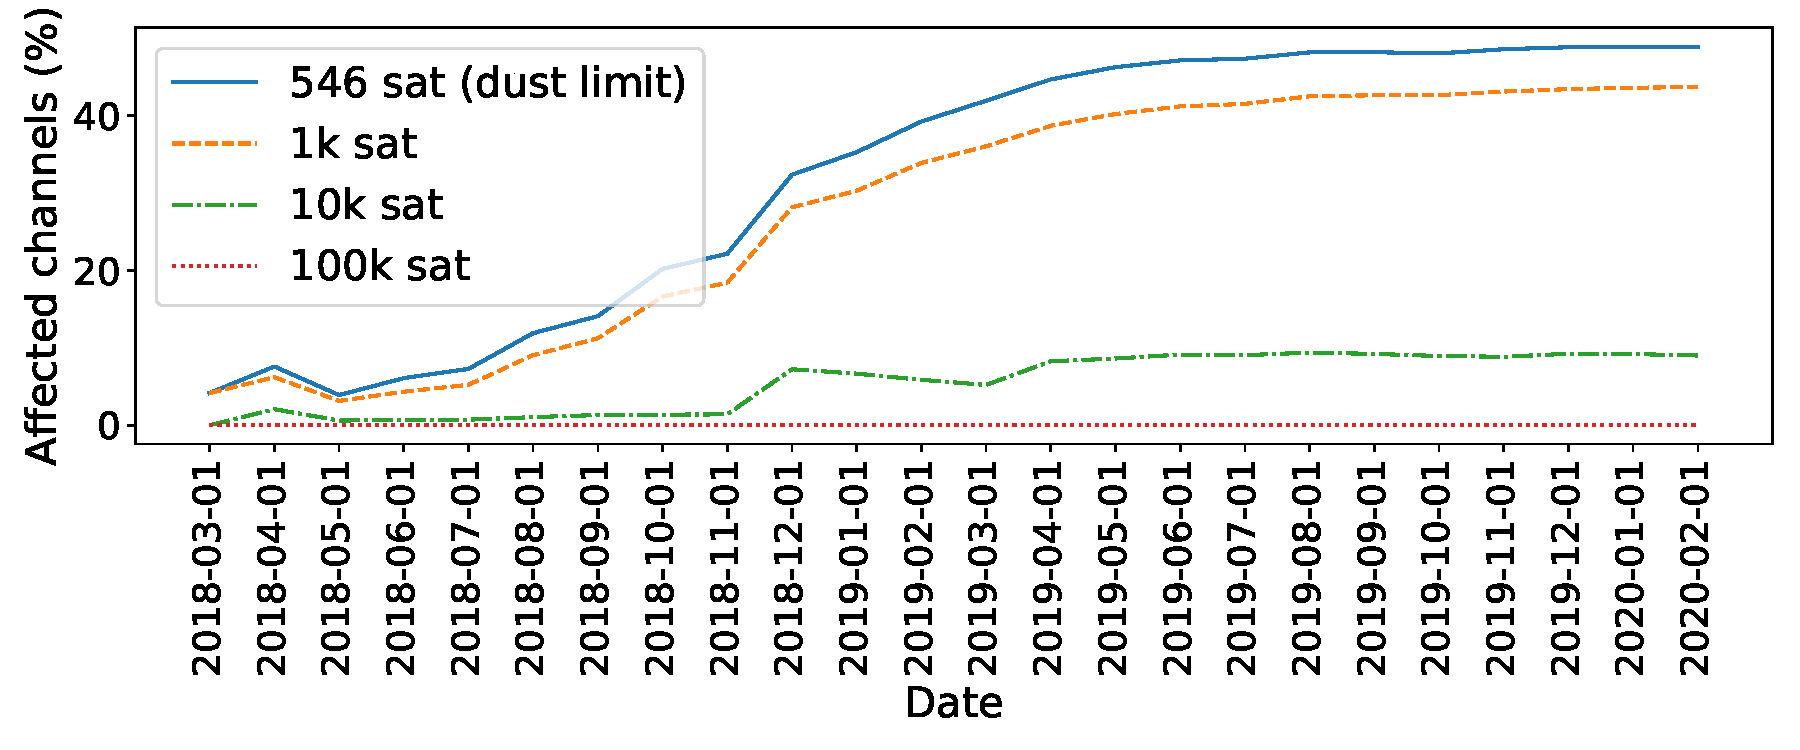
\includegraphics[width=\columnwidth]{historic-htlc-limited-share}
	\caption{Historic share of HTLC-limited channels.\label{fig:historic-htlc-limited-share}}
\end{figure}

\begin{figure}[tb]
	\centering
	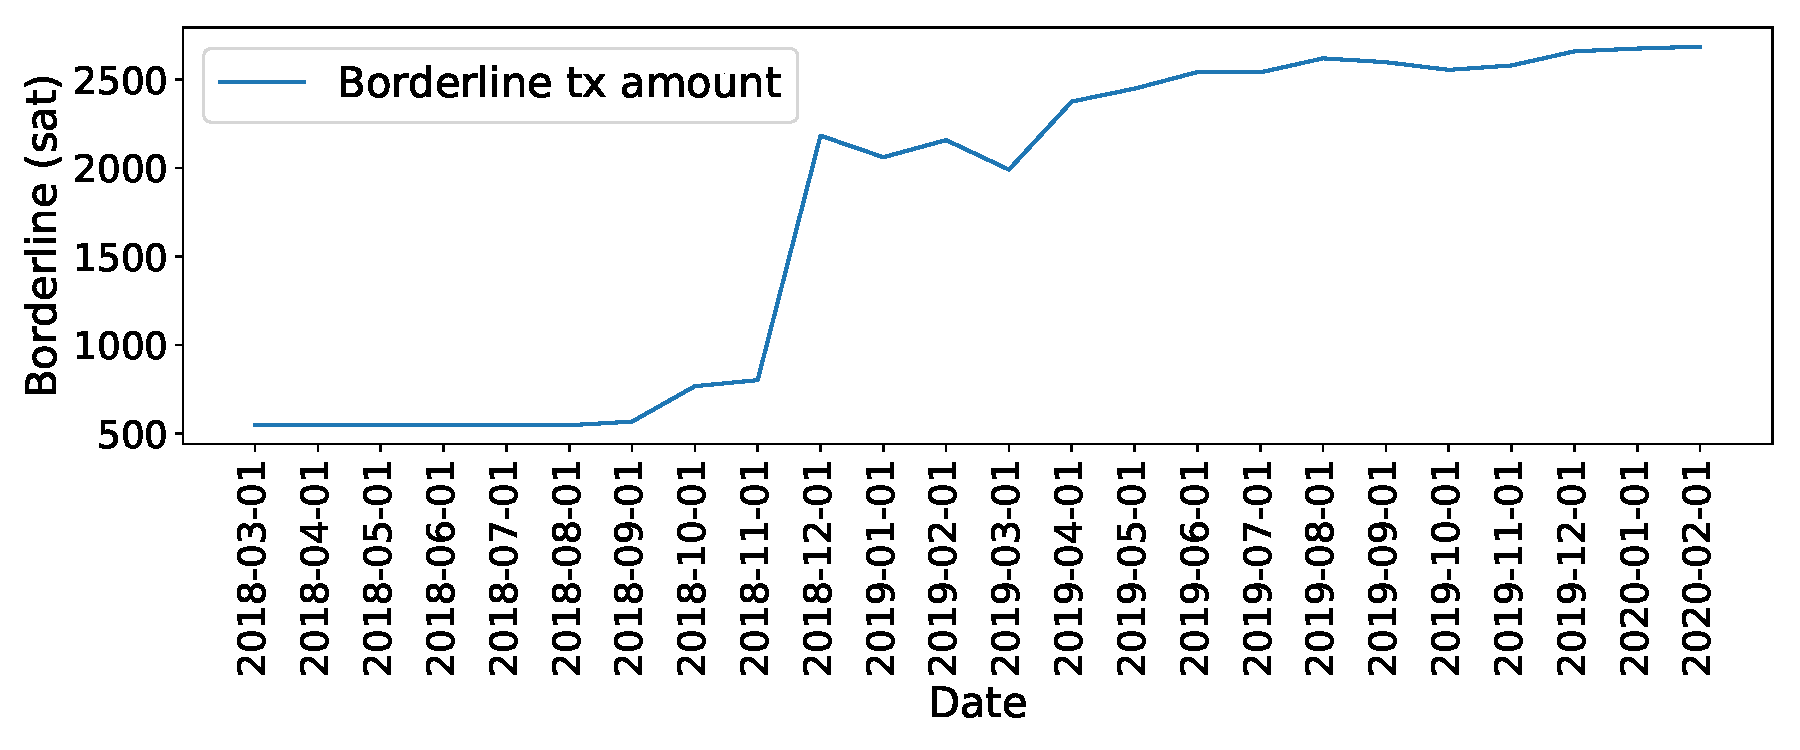
\includegraphics[width=\columnwidth]{historic-borderline-amount}
	\caption{Historic borderline amounts.\label{fig:historic-borderline-amount}}
\end{figure}



\subsection{Depleting the Lightning Network}

The HTLC limit opens up the possibility of a network-wide DoS attack.
An adversary connects to both endpoints of the target channel and forwards multiple small payments to itself, 
but does not finalize them.
After $966$ HTLCs are added, the channel loses its ability to forward payments, until some HTLCs expire. 
The attacker can thereby deplete a channel, making it unusable.

The cost for this attack depends on the minimum transaction amount.
% allowed by the channel and the dust limit.
%These values are set at the time of channel creation and can be later modified by the counterparties.
%From our dataset \textit{LN20}, the average minimum transaction amount is $1.273$~satoshis.
%Only $61$ out of more than $62$~thousand channel endpoints declare a minimum transaction amount higher than $1$~satoshi (the default setting in popular LN implementations).
We assume it equal to the dust limit of $546$~satoshis (the default value in 2 out of 3 major implementations).

We calculate the total capital requirements for an attacker to block the complete LN.
To block all $31084$~channels, the attacker would send, in the worst case, $966$ transactions of $546$ satoshi to each channel.
This brings the total capital requirements to approximately $163.9482$~BTC ($1.64M$~USD).

Each HTLC defines a timeout, after which the funds are returned to the sender, if the receiver provides no preimage.
From our dataset, we see that HTLC timeouts are long: $75.44$ blocks on average.
At a block creation rate of $10$~minutes per block, this implies that an average HTLC can block the capacity for around $12$~hours.
This implies that the attacker can render channels useless for around $12$~hours using the same HTLC parameters as regular LN users.
% Re-calculated in SQLite, 2020-02-25 data
%\todo[inline]{Pedro: These 12 hours number needs to be explained. Sergei: explained, is it OK?}


While this rough upper bound estimate suggests a rather high attack cost, the following optimizations make it more affordable.


\subsubsection*{Targeting highest-capacity channels}
The attack impact can be maximized by targeting highest-capacity channels.
For example, it requires $0.05$~BTC to block 10~top channels with combined capacity of $17.91$~BTC (\cref{fig:block-top-channels}).

\begin{figure}[tb]
	\centering
	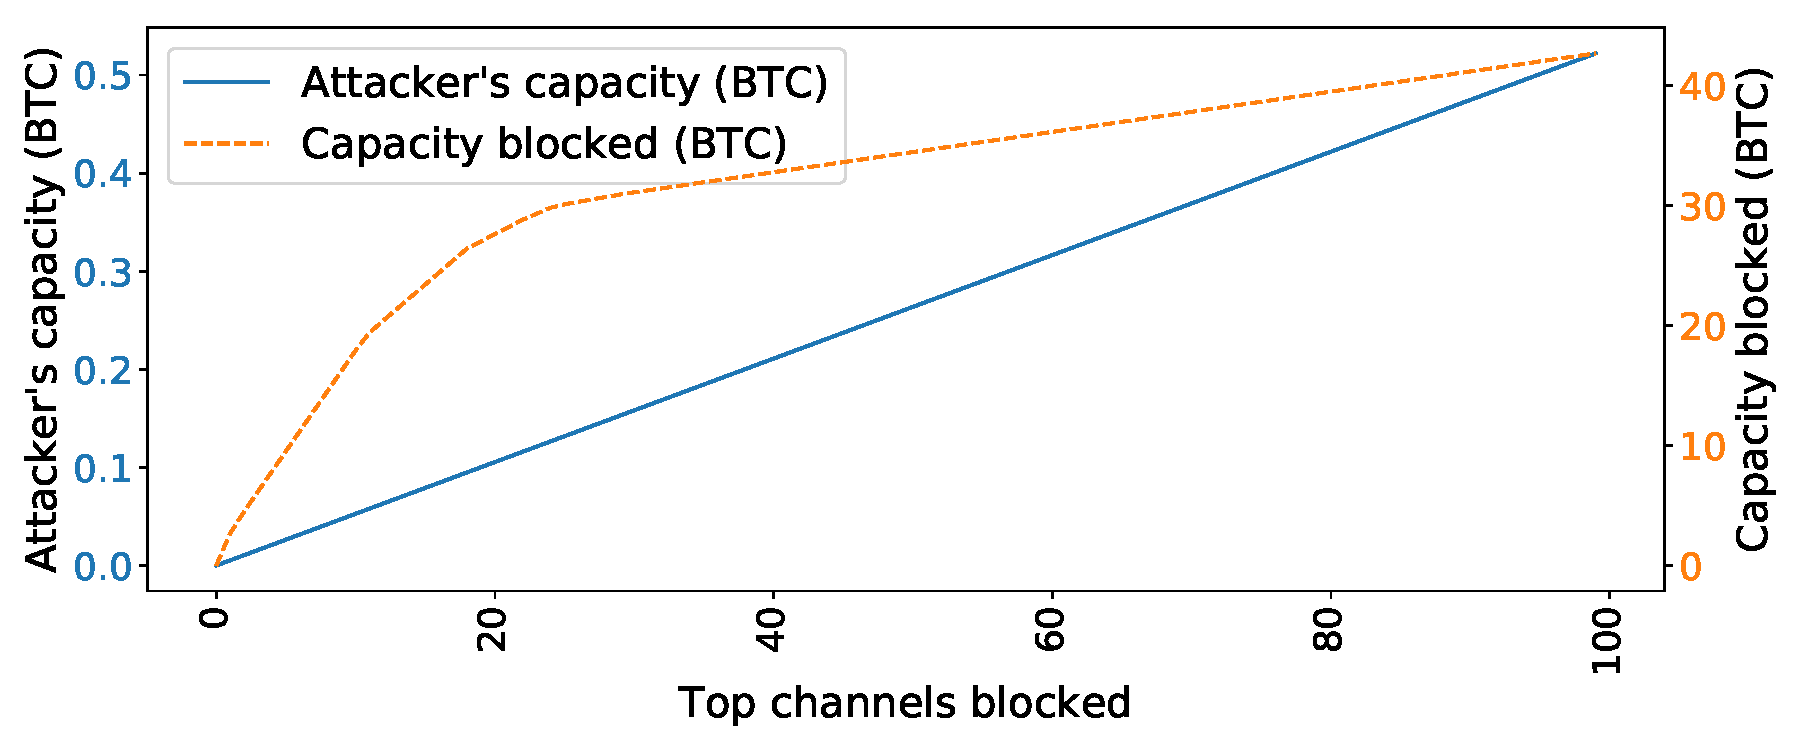
\includegraphics[width=\columnwidth]{block-top-channels}
	\caption{Effectiveness of targeting highest-capacity channels.\label{fig:block-top-channels}}
\end{figure}

\subsubsection*{Real HTLC limit}
Our calculations above are based on the maximum number of concurrent HTLC as defined by BOLT specifications ($483$).
LN implementations may choose lower default values for this parameter.
In particular, Eclair and c-lightning enforce a lower default HTLC limit ($30$).
%The third major implementation -- LND -- supports $483$~concurrent HTLCs per channel.
This means that in the real network the attacker needs to create fewer HTLCs to block channels between c-lightning and Eclair nodes as opposed to theoretical calculations and LND nodes (which by default support $483$ concurrent HTLCs per channel).
LND makes up $91\%$ of the nodes in the network, and Eclair is another $1\%$~\cite{Mizrahi2020}.
That brings real average HTLC limit to $442.23$ and lowers the attack cost by~$8.44\%$.
%\todo[inline]{Pedro: I don't understand this paragraph. Sergei: Now it's good?}

\subsubsection*{Multi-hop transactions}
The estimation above assumes single-hop transactions.
An attacker can leverage multi-hop transactions to multiply the effect of the committed capital,
connecting to both ends of a $20$-hop~\cite{Bolt4OnionRouting} payment path and performing a payment 
to itself that never gets completed. 
This is similar to capacity-based griefing attacks~\cite{HerreraJoancomarti2019}, 
but with much lower capital requirements.

\subsubsection*{Optimizing the attack based on communities}
The attacker may wish to prevent different parts of the network from transacting to each other.
To evaluate this possibility, we first divide the network into \textit{communities} using the Clauset-Newman-Moore greedy modularity maximization algorithm~\cite{Clauset2004}.
%LN graph can be divided into 25~communities.
Then we consider a scenario where the attacker tries to block the channels that connect communities 
rather than channels within communities.
For a chosen number $N$ of the largetst communities, we calculate how many channels the attacker has to block to split the network into at least $N+1$ parts: the $N$ largest communities and the rest of the network (\cref{fig:isolate-communities}).
We observe, e.g.,~that the attacker needs to block $4670$ channels 
($13\%$~of all channels) to isolate the largest community from the rest of the network, locking up $25$~BTC ($225k$~USD) -- or just around $2.8\%$~of the total LN capacity.
%\todo[inline]{Pedro: This number is a little discouraging. Shall we put it as a percentage of the total capital in the LN instead?}

\begin{figure}[tb]
	\centering
	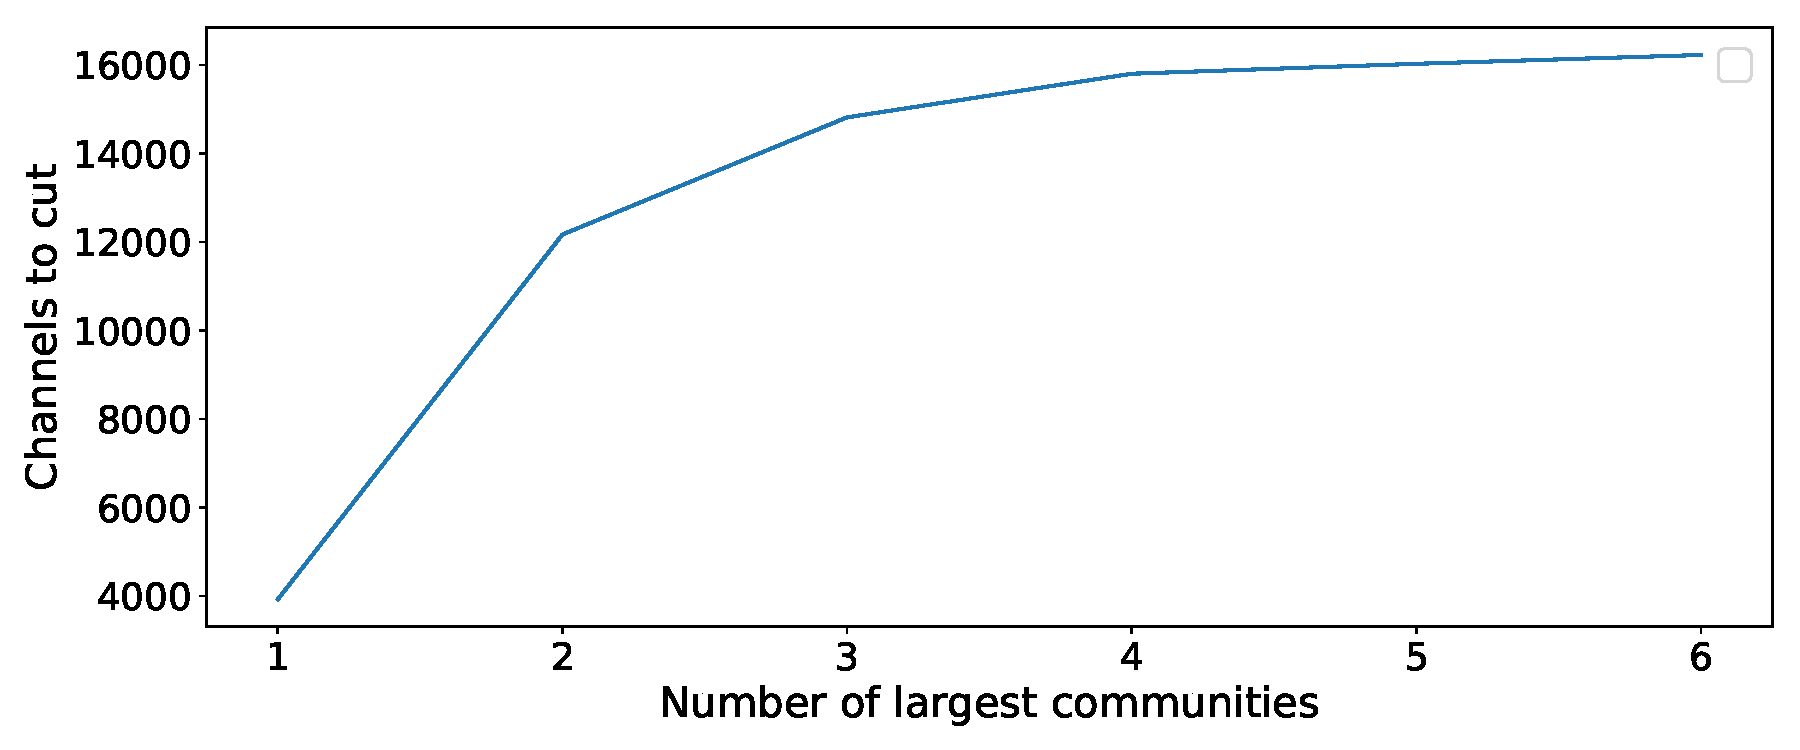
\includegraphics[width=\columnwidth]{isolate-communities}
	\caption{Number of channels to cut to isolate the largest communities.\label{fig:isolate-communities}}
\end{figure}



\subsection{Discussion}
Our simplistic model does not fully reflect all the details of transaction handling. 
In particular, we do not account for the fact that transactions take multiple hops (and multiple failed paths) before succeeding, nor do we reflect the unequal forwarding ability of a unit of capacity at a well-connected node, 
as opposed to a poorly connected one.
We also do not account for non-public channels, which may account for $28\%$~of all channels~\cite{BitMEXPrivateChannels}.
Yet, our approach allows us to calculate the effect of the HTLC limit,
as both estimations (capacity-based limit and HTLC limit) are calculated under the same assumptions.
Our estimation shows that the HTLC limit reduces the number of concurrent channel updates 
for payments under certain average transaction amount. 

The fact that the HTLC limit manifests itself at low transaction amounts negatively affects scalability.
Many potential LN applications involve transactions with tiny amounts.
The original Lightning paper~\cite{Poon2016} envisions use cases such as paying for online content and internet traffic.
Our calculations show that for payments of $1000$~satoshis ($0.009$~USD),
the network-wide rate of concurrent channel updates is $60\%$ lower 
than it could have been based solely on capacity limitations.

The low value for the default minimum transaction amount and the reduced number of in-flight transactions  
open a DoS attack vector with a moderate cost for the adversary.
Note that the capital in the attacker's channels will be recouped after the HTLCs time out.
Moreover, the unequal distribution of connectivity in the current LN paves the way for optimized attacks 
where the attacker focuses on high-capacity or inter-community channels to disrupt the 
seamless transfer of value across the network.


\subsection{Countermeasures}
One of the limiting factors for transaction throughput is the total available capacity.
This limitation is overcome by opening new channels, 
a countermeasure that will be naturally implemented with the growing LN adoption. 
The issue of the HTLC limit is more challenging as it comes from the limitations of the Bitcoin and Lightning protocols themselves.
Therefore, more fundamental changes are needed to reduce the information required to  
carry out the functionality encoded in HTLCs.
One countermeasure involves replacing HTLC with AMHL~\cite{Malavolta2019}. 
While HTLC requires including a digital signature, a hash value and a timelock, AMHL contract only requires the digital signature and the timelock while providing the same functionality. 

%Another potential countermeasure is the planned Taproot update to Bitcoin~\cite{TaprootBIP}.
%This update would allow to implement the HTLC functionality more compactly using Schnorr signatures.
%\todo[inline]{Pedro: We could add taproot here.Sergei: is this accurate?}

This countermeasure would reduce the number of bytes required per in-flight transaction 
and increase the number of payments handled concurrently.
While not removing the limitation on the number of concurrent transactions, 
this countermeasure raises this limit, reducing its negative effect on LN scalability.



\section{Related work}
\label{sec:related-work}

%We can roughly divide the related literature in two groups: academic analyses of the concept of payment-channel networks (PCN)
%and experimental analyses of the Lightning Network data.

Multiple research works have shed light on various aspects of payment-channel networks, such as security~\cite{Malavolta2019, Kiayias2019}, privacy~\cite{Malavolta2017, HerreraJoancomarti2019}, concurrency~\cite{Malavolta2017}, routing~\cite{Malavolta2017a, Roos2018, Sivaraman2018, Prihodko2016}, liquidity~\cite{Dandekar2011,MorenoSanchez2018}, efficiency~\cite{Decker2018}, and incentive compatibility~\cite{Engelmann2017}.
These works mainly share the lack of a quantitative analysis of the impact of their findings in the current LN.
%In tour work , we have empirically analyzed the potential severity of the wormhole attack, 
%as well as attacks on value privacy and relationship anonymity, in the current Lightning Network. 

A group of papers more closely related to ours conveys experimental analyses of various aspects of the LN.
Herrera-Joancomart\'{i} et al.~\cite{HerreraJoancomarti2019} describe an adversarial 
strategy to determine the current balance of a channel in the network.
Tang et al.~\cite{Tang2019} study 
the tradeoffs between balance privacy and routing effectiveness. 
Martinazzi~\cite{Martinazzi2019} and Seres et al.~\cite{Seres2019} study the evolution of topological aspects of the LN graph.
Conoscenti et al.~\cite{Conoscenti2019} study the dependency of the LN on payment hubs 
and the rebalancing mechanisms that ameliorate the effect of depleted channels.
Tochner et al.~\cite{Tochner2019} analyze a DoS attack vector based on route hijacking. 
P{\'{e}}rez{-}Sol{\`{a}} et al.~\cite{PerezSola2019} introduce the LockDown attack where the adversary 
prevents a LN node from transacting by depleting the capacity in all its channels.
In comparison, our HTLC depletion attack achieves the same result (a victim node can not forward payments), but exploits the HTLC limit at each channel rather than its capacity.
%\todo[inline]{Pedro:I would not put this text in a footnote. We need to say why related work is different from this}
%Our experiments show that the isolation of a node (or part of a network) 
%exploiting the HTLC limit is cheaper for the adversary than the attack proposed by P{\'{e}}rez{-}Sol{\`{a}} et al. 
Finally, concurrently to our research, Mizrahi and Zohar~\cite{Mizrahi2020} study the HTLC limit and its effects.
Their work, however, does not account for the way LN handles payments below the dust limit.
%\todo[inline]{Pedro: Same here. What's the difference with this work? Aren't they missing the point that 1satoshi payments are not carried out with HTLC?}


%their estimated cost of attacking one node is $15$~EUR ($16.5$~USD), whereas the cost of attacking the whole LN in our case is estimated at $3000$~USD, i.e.,~around $0.6$~USD per node.


\section{Conclusions}
\label{sec:conclusions}

The Lightning Network (LN) has emerged as the most widely deployed solution for the scalability issue affecting current blockchains such as Bitcoin. 
%Its substantial growth in the number of nodes, payment channels and their capacity has attracted attention from academia and industry.
Despite its conceptual appeal and growing adoption,  several works~\cite{Malavolta2017, Malavolta2019} have identified 
 security, anonymity and scalability limitations. A quantitative 
analysis of their impact, however, is missing and this paper aims at filling this gap.

We quantitatively study for the first time the proneness of the current Lightning Network to the 
wormhole attack as well as attacks against value privacy and relationship anonymity. 
We observe that a moderately resourceful adversary controlling only $2\%$ of the total node count can carry out these attacks with high success probability.

We also quantitatively analyze the negative effect on scalability produced by the limit on concurrent payments in the LN. 
We calculate that the limited concurrency in the LN implies that an adversary can block the complete LN investing around $1.5M$~USD ($18.5\%$~of the network capacity), and this cost can be substantially reduced by targeting highly valuable channels (e.g., high-capacity channels or those connecting the biggest communities in the network).
%\todo[inline]{Pedro: This is not an encouraging conclusion :)}

%First, we quantitatively analyze the effect of the wormhole attack as well as attacks on value privacy and relationship anonymity. 
%Second, we quantitatively analyze the restriction of the LN scalability gain due to the limited concurrency supported by the LN protocol. 
%In particular, we observe that more than up to $50\%$ of LN channels can support fewer concurrent micropayments than in principle allowed by their capacity. 
%For instance, the adversary investing $225$k~USD can prevent nodes in the largest community from transacting with the rest of the network. 

% the probability of three privacy attacks depending on payment amounts and the number of compromised nodes.
%Our results show that a payment's probability of being forwarded through a malicious path does not depend on its size, but large payments are less likely to succeed at all.
%Among the three attacks we considered, value privacy is the most sensitive to the number of compromised nodes.
%With just a few highly-connected hubs compromised, LN users risk having their payment amounts leaked to the adversary.
%Relationship anonymity attack and, finally, the wormhole attack are less likely with the same number of malicious nodes.

%Then, we have described an understudied drawback of LN -- the limit on the number of concurrent in-flight payments (HTLCs) in a channel.
%This limitation is explained by the interaction between Lightning and Bitcoin protocols.
%We have shown, first, that this is the key factor limiting LN performance for small payments.
%Our results indicate that some of the widely discussed LN use cases (such as micropayments) might not be viable even with sufficient channel capacity.
%We describe a DoS attack vector based on the HTLC limit and show that it is more efficient for the attacker to block channels by depleting their HTLC limit rather than capacity, as has been already described in the literature.
%In this state of affairs, we prompt the LN community to implement countermeasures to alleviate these security, anonymity and scalability issues. 
%For instance,  we argue that implementing anonymous multi-hop locks (AMHL) instead of the currently used HTLC construction would 
%mitigate the security, privacy  and scalability issues.  %We hope that this work helps Lightning and Bitcoin communities identify and address the most pressing bottlenecks of these technologies and help them achieve their full potential.

